%% Language and font encodings
%% Sets page size and margins
%% Useful packages

\documentclass[a4paper]{article}%
\usepackage[english]{babel}
\usepackage[utf8x]{inputenc}
\usepackage[T1]{fontenc}
\usepackage{subcaption}
\usepackage[font={small,it}]{caption}
\usepackage{graphicx}
\usepackage[a4paper,top=3cm,bottom=1.5cm,left=1.5cm,right=1.3cm,marginparwidth=1.30cm]%
{geometry}
\usepackage{amsfonts}
\usepackage{amsmath,bm}
\usepackage{svg}
\usepackage{graphicx}
\usepackage{xcolor}
\usepackage[english]{fancyref}
\usepackage{authblk}
\usepackage[autostyle]{csquotes}
\usepackage[colorinlistoftodos]{todonotes}
\usepackage[colorlinks=true, allcolors=blue]{hyperref}
\usepackage{natbib}
\usepackage{graphicx}
\usepackage{amsmath}
\usepackage{amssymb}%
\setcounter{MaxMatrixCols}{30}
%TCIDATA{OutputFilter=latex2.dll}
%TCIDATA{Version=5.50.0.2960}
%TCIDATA{LastRevised=Monday, November 09, 2020 20:09:17}
%TCIDATA{<META NAME="GraphicsSave" CONTENT="32">}
%TCIDATA{<META NAME="SaveForMode" CONTENT="1">}
%TCIDATA{BibliographyScheme=BibTeX}
%TCIDATA{Language=American English}
%BeginMSIPreambleData
\providecommand{\U}[1]{\protect\rule{.1in}{.1in}}
%EndMSIPreambleData
\DeclareCaptionLabelFormat{adja-page}{\hrulefill\\#1 #2 \emph{(previous page)}}
\newcommand{\norm}[1]{\left\lVert#1\right\rVert}
\DeclareMathOperator*{\argmin}{arg\,min}
\DeclareMathOperator*{\argmax}{arg\,max}
\DeclareMathOperator\erf{erf}
\DeclareMathOperator\erfc{erfc}
\begin{document}

\title{\vspace{-5em} Compressed Coding in a Shallow Neural Network with Random Weights}
\author{

}
\date{}
\maketitle

\section{Summary}

The mean response of neurons to parameters of sensory stimuli is characterized
by tuning curves. Classically, these response profiles are described
by simple, monomodal or monotonic, smooth functions. Interesting coding
properties emerge with more complex tuning curves: as an example,
grid cells, with their spatially periodic responses, generate a
precise code \cite{Sreenivasan2011GridComputation}. These multi-peaked tuning
curves allow for combinatorial patterns of activity to represent
spatial locations with fewer neurons than in a population
with monomodal tuning curves.

Is periodicity necessary for enhanced coding, or do similar
properties emerge more generally in populations of neurons with
complex tuning curves? To address this question, we consider
a simple circuit that produces complex but unstructured tuning curves, namely,
a feedforward neural network with random connectivity, in which
information is compressed from a first layer to a second one of smaller size.
The random connectivity generates irregular tuning curves; these
represent richer `sensors' of the stimulus (as compared to monomodal
tuning curves), but result in ambiguous coding which can yield catastrophic
errors. Combining analytical and numerical methods, we show that, as a
function of its parameters, this simple network interpolates between a
classical code robust to noise and a combinatorial code, highly accurate but
prone to catastrophic errors. Efficient coding implies an optimal point that
specifies the spatial scale of tuning curve irregularities, as a function of
the compression of the information between network layers.

Spatial coding in the monkey motor cortex can be viewed as an
instantiation of such a `compressed coding'. We reanalyze earlier data
\cite{Lalazar2016TuningConnectivity} by extending our model to
higher-dimensional stimuli and fitting it to neural recordings. The approach
enables us to compare the performance of a compressed coding model of spatial
representation in motor cortex with the classical model that assumes smooth,
linear tuning curves. This example illustrates the possible use of complex
tuning curves in population coding. More generally, our work proposes a new
angle on efficient population coding beyond the classical model with simple
tuning curves.

\section{Additional details}

Tuning curves are used broadly in neuroscience to describe
the response of neurons to parameters of sensory stimuli. Their shape is often
described by simple, smooth functions, like Gaussians or sigmoids,
and a large body of literature addresses the problem of optimizing
the parameters of these functions with respect to an objective or loss
function such as the estimation error \cite{Zhang1999NeuronalBroaden}.
In classical models, this error is small in large populations of
neurons; typically, it decreases as an inverse power of the population size.

%% More efficient coding schemes
However, more efficient coding schemes exist in terms of error suppression
with the size of the population. A paradigmatic example is given by grid cells
in the entorhinal cortex, which collectively encode the position of an animal
moving in an environment by means of spatially periodic tuning curves with
different periods. Sreenivasan and Fiete \cite{Sreenivasan2011GridComputation}
showed how in such populations the error in the position estimate decreases
exponentially with the number of neurons, thus outperforming classical codes.
This phenomenon can be intuited from a geometrical representation
introduced by Shannon 
\cite{Shannon1949CommunicationNoise}, on the basis of which a coding scheme
can be regarded as a map that associates each realization of the stimulus with
a point in the space of the joint neural activities of the population. For a
population of grid cells, due to the periodicity of their responses,
fully combinatorial patterns of activity actually 
 correspond to  encoded stimuli. This results in a
denser coverage of the activity space and, consequently, in a more
accurate local representation of the encoded sensory variable as compared to
the case of an equisized population of classically tuned neurons.
However, this coding scheme comes with the drawback that two
distant stimuli can be mapped to nearby activity patterns and
thereby become indistinguishable due to the presence of noise that
corrupts neural responses. As a result, in such a code, large or
`global' errors in stimulus estimation can occur.

%% The model
While grid cells are widely studied in the literature, there may be other
coding schemes that share similar coding properties. In order to see
if a highly designed structure as periodicity is necessary
for enhanced coding, we consider a two-layer feedforward
neural network with unstructured, i.e., random, connectivity. In the
first layer, a large population of $L$ sensory neurons encodes a
one-dimensional stimulus into a high-dimensional representation by
means of Gaussian tuning curves of width $\sigma$, whose centers are
arranged uniformly over the stimulus space. This population projects
onto a smaller layer of $N$ neurons by means of random i.i.d. synaptic
weights, which effectively generate a set of irregular tuning curves
in the second layer. The average  joint activity of neurons in this
layer, as parametrized by the stimulus, can be represented as a
one-dimensional manifold embedded in the $N$-dimensional
space of neural responses (Fig.\ref{Fig:cosyne_abstract}). \textbf{We model the trial to trial variability as i.i.d Gaussian noise; this noise will perturb the responses away from this manifold.} The tuning
width, $\sigma$, of neurons in the first layer
 governs the scale of the irregularities
in the manifold, that is, the extent to which responses
preserve the distance between two nearby stimuli. If $\sigma$
is small, neurons in the second layer generate uncorrelated random responses
regardless of the distance between stimuli, and the manifold
reduces to an ensemble of scattered points in the activity
space. As $\sigma$ grows, irregularities are smoothed
out, and nearby stimuli evoke increasingly correlated responses.

\textbf{In order to study the coding properties of the network, we quantified the coding accuracy through the Mean Square Error (MSE)  in the stimulus estimate as obtained from an
ideal decoder. This decoder will associate to each noisy response, the stimulus corresponding to the closest point on the manifold. }We showed that the error can be viewed as the sum of two
qualitatively distinct contributions:
\begin{equation}
\varepsilon^{2}=\varepsilon_{l}^{2}+\varepsilon_{g}^{2}.\label{Eq:LvsG}%
\end{equation}
`Local errors', quantified by $\varepsilon_{l}^{2}$, occur
when estimates are close to the true stimulus value; this kind of
error scales with the tuning width,  $\varepsilon_{l}\sim\frac
{\sigma}{N}$, and the tuning width in turn rules the local curvature
of the manifold. `Global errors' are controlled by
the winding of the response manifold, and scale as
$\varepsilon_{g}\sim\frac{1}{\sigma}\exp{(-N)}$. In a regime of
compression, i.e.,  when $N\ll L$, there is a trade-off
between $\varepsilon_{l}$ and $\varepsilon_{g}$ that yields optimal tuning
parameters, for which the total error us suppressed exponentially with
population size. We corroborated the analytical results with
numerical simulations; .

Spatial coding in monkey motor cortex can be viewed as an
instantiation of the coding scheme just outlined. During a \textbf{[static
task -- ???]}, neurons in this area encode the spatial position of the
monkey's hand; classically, their responses have been
fitted to a function  of the
cosine of the angle between the target position
and a `preferred direction', that varies from neuron to neuron.
In a recent study, Lalazar et al.
\cite{Lalazar2016TuningConnectivity} proposed a new fit of tuning
curves that took into account the heterogeneity among neurons
on a finer scale. Motivated by the similarity of their model with a
generalization of our shallow random network that encodes a three-dimensional
stimulus, we used the latter to capture the monkey cortex data.
Despite being simpler, our model yielded a faithful fit of the neural
recording; it also allowed us to quantify spatial coding in cortical
populations of neurons, and, in particular, to compare coding when tuning
curves take their classical, simpler form and the more complex form generated
in our network. By varying the population size and the magnitude of
the single-neuron noise, we identified the parameter regions in which tuning
curve irregularities are beneficial to spatial coding, in spite of
the ambiguity that they may generate.
Our work illustrates the power of complex tuning curves and compressed
coding in the absence of a highly structured design of a network, and
suggests, correspondingly, that a brain area achieve a balance between high
encoding accuracy and robustness to noise.

\begin{figure}[ptb]
\centering
\includegraphics[width=\textwidth]{cosyne_abstract.eps}\caption{\textbf{Geometrical
view of a random coding scheme.} {Example of manifold described by the joint
activity of three neurons, for increasing value of $\sigma$. The three axes
represent the firing rate of three sample neurons and the manifold is color
coded according to the corrsponding stimulus value as shown in the legend.
Trial to trial variability in the population response is represented as a grey
cloud of noisy responses around the mean value. By lowering $\sigma$ , the manifold increases in length, resulting in higher discrimination of stimuli inside the same ball. On the other hand, the probability that the ball includes segment of the manifold coding for distant stimuli, represented by different colors, is higher.}%
\label{Fig:cosyne_abstract}%
\end{figure}

\bibliographystyle{unsrt}
\bibliography{references}

\end{document}